\section{Selected} \label{sec:Selected}

This utility creates a new coordinate file. By default, the utility saves all
bead and molecules types (basically transforming one coordinate file format into
another), but using \tt{-bt} and/or \tt{-mt} options specifies which bead and/or
molecule types to exclude from the output file. If \tt{--keep} option is used,
the specified bead and/or molecule types are instead the only ones that are
written into the output file.

Besides the standard \tt{-st}, \tt{-e}, and \tt{-sk} options, which timesteps to
save can be explicitly specified via the \tt{-n} option that can take a maximum
of 100 arguments (the \tt{-st}, \tt{-e}, and \tt{-sk} are then ignored). Also,
using \tt{--last} option saves only the last valid step from the input
coordinate file (all the previous options are ignored if \tt{--last} is used).
If LAMMPS \data file is used as a coordinate file, all the above options are
ignored as the \data file contains by definition only a single timestep.

There is also an option to remove periodic boundary conditions for molecules
(i.e., to \enquote{join} them) via the \tt{--join} switch. Conversely, the
simulation box can be wrapped (i.e., the periodic boundary conditions applied,
putting all beads inside the box) via the \tt{--wrap} switch. If both
\tt{--wrap} and \tt{--join} options are used, the simulation box is first
wrapped and then the molecules are joined.

\begin{figure}[b]
  \centering
  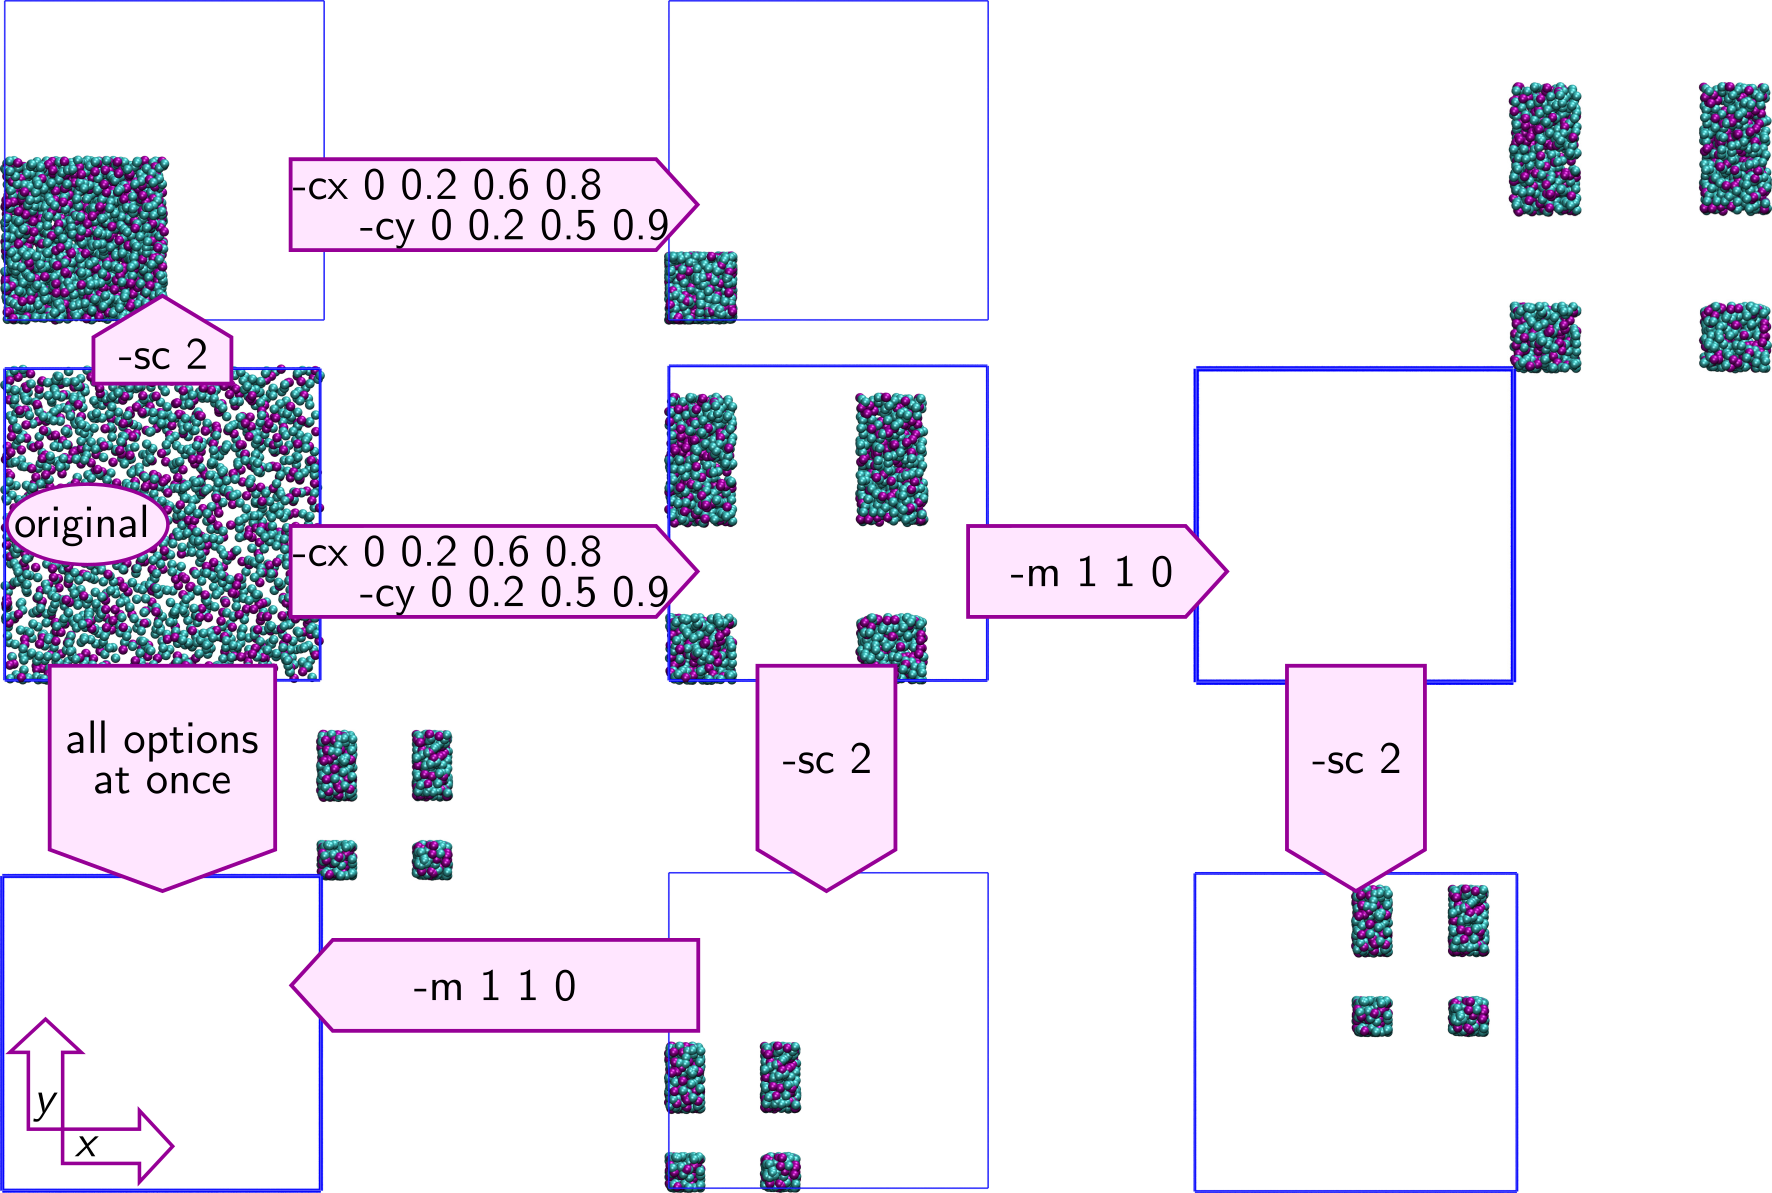
\includegraphics{Selected.png}
  \caption{
    Some of the possible results when combining sequential runs of the
    \tt{Selected} utility, namely (1) constraining $x$ and $y$ coordinates via
    \tt{-cx 0 0.2 0.6 0.8 -cy 0 0.2 0.5 0.9}, (2) scaling (dividing) coordinates
    via \tt{-sc 2}, and (3) moving coordinates via \tt{-m 1 1 0}.
  }
  \label{fig:Selected}
\end{figure}

Furthermore, some basic manipulations of the coordinates are possible:
\begin{enumerate}
  \item using \tt{-cx}, \tt{-cy}, and/or \tt{-cz} options, only beads whose
    coordinates fit the constraints are considered for saving (see below for
    what \enquote{fit} means)
  \item using \tt{-sc <float>} option scales coordinates by dividing them by
    \tt{<float>}
  \item using \tt{-m 3×<float>} option moves all coordinates by the given vector
\end{enumerate}

Both \tt{-cx/y/z} and \tt{-m} options accept fractions of box size (i.e.,
numbers between 0 and 1) by default. To specify \enquote{real} coordinates
instead, use the \tt{--real} option. The output simulation box remains
unchanged, and the resulting coordinates may be outside the box. The \tt{--wrap}
and \tt{--join} options are applied after these manipulations.

The constraining options accept multiples of number pairs for each axis; a bead
coordinate must fall within at least one of the ranges, e.g., using \tt{-cx 0
0.1 0.9 1} would save beads whose $x$ coordinates are within 0 to 10\% or 90\%
to 100\% of the box size in the x-direction. Adding, e.g., \tt{-cy 0.4 0.6}
would save only the beads that fulfil the \tt{-cx} option as well as this one,
i.e., that $y$ coordinate is between 40\% and 60\% of the simulation box.

Note that when a combination of these options is provided, the manipulations
happen in the numbered order, e.g., using all three types of options,
the coordinates are first constrained via \tt{-cx/y/z} option(s), then all
coordinates are scaled via \tt{-sc}, and finally, the coordinates are moved
via \tt{-m}. This is represented in \cref{fig:Selected} by going from the
\enquote{original} system straight down. The sequence
\enquote{original}-right-down-left shows it is the same as running three
\tt{Selected} command in sequence. \Cref{fig:Selected} also shows examples of
what can happen when \tt{Selected} commands are run in sequence with different
options. The \tt{Selected} commands to generate these examples are in the
\tt{Examples/Selected} directory.

\vspace{1em}
\noindent
Usage: \tt{Selected <input> <output> <bead type(s)> [options]}
\noindent
\begin{longtable}{p{0.22\textwidth}p{0.724\textwidth}}
  \toprule
  \multicolumn{2}{l}{Mandatory arguments}\\
  \midrule
  \tt{<input>}        & input coordinate file\\
  \tt{<output>}       & output coordinate file\\
  \midrule
  \multicolumn{2}{l}{Options}\\
  \midrule
  \tt{-bt <bead type>} & bead types to exclude\\
  \tt{-mt <mol type>}  & molecule types to exclude\\
  \tt{--keep}          & save only specified types instead of excluding them\\
  \tt{--join}          & join molecules by removing periodic boundary
                         conditions\\
  \tt{--wrap}          & wrap simulation box (i.e., apply periodic boundary
                         conditions)\\
  \tt{-n <int(s)>}     & save only specified timesteps\\
  \tt{--last}          & save only the last step\\
  \tt{-sc <float>}     & divide all coordinates by given value\\
  \tt{-m 3×<float>}    & add specified vector to all coordinates (\tt{-sc} is
                         applied first)\\
  \tt{-cx n×2×<float>} & constrain x-coordinates to specified dimension;
                         multiple pairs possible\\
  \tt{-cy n×2×<float>} & same as \tt{-cx} but with y-coordinates\\
  \tt{-cz n×2×<float>} & same as \tt{-cx} but with z-coordinates\\
  \tt{--real}          & use real coordinates instead of fractions of box size
                         (for \tt{-cx/y/z} and \tt{-m} options)\\
  \midrule
  \multicolumn{2}{l}{Other options (see the beginning of
                     Chapter~\ref{chap:Utils})}\\
  \midrule
  \multicolumn{2}{p{0.948\textwidth}}{\tt{-st},
                                      \tt{-e},
                                      \tt{-sk},
                                      \tt{-i},
                                      \tt{--verbose},
                                      \tt{--silent},
                                      \tt{--help},
                                      \tt{--version}}\\
  \bottomrule
\end{longtable}
